% PART 2

\section{Prevalence of Improper De-identification Methods: A Review of ``Non-identifiable'' Datasets used in Australian Rules Football Research}
\label{ch:ethics-details}

% Supervisor: {May be better in prose}
% \as {Can convert to prose in final thesis, but leaving as is for now so to we can submit as an abstract to a sport science / medical journal)}

\subsection{Abstract}

% \newcommand{\hs}{\hspace{1em}} % moved to preamble

\textbf{Background}\hs Non-identifiable datasets are afforded special exemptions under privacy law and human research regulations. For a dataset to be made \textit{non-identifiable}, it must undergo a de-identification process to ensure that ``no specific individual can be identified'' \cite{NationalStatement2015}. Stripping personally identifying information while leaving other fields is now a ``discredited approach'' \cite{Ohm2010} due to the risk of linkage in data-rich environments. De-identified sport datasets, particularly GPS tracking datasets, involve spatio-temporal microdata that may be vulnerable to re-identification.

\textbf{Objectives}\hs To determine the prevalence of improper de-identification methodologies used in Australian Rules Football research.

\textbf{Data sources}\hs Electronic literature search using Google Scholar to sample both academic and grey literature.

\textbf{Study eligibility criteria}\hs Study involves collection or use of data related to Australian Rules Football, and makes a claim about the identifiability status of players or teams in the data.

\textbf{Study appraisal and synthesis methods}\hs Re-analysis of all variables collected from the perspective of re-identification attacks, particularly data linkage attacks.

\textbf{Results}\hs In two of three studies, the underlying research dataset was claimed to be non-identifiable, but included identifying attributes that could have revealed non-public information about participants. None of the studies allowed re-identification of the participants on the basis of published data alone.

\textbf{Conclusions}\hs The de-identification approaches prevalent in sport research provide the illusion of de-identification, but offer no protection against deliberate re-identification attempts. Sport researchers and Human Ethics Advisory committees should not declare data \textit{non-identifiable} without consideration of re-identification attacks that may link records to the ever-growing body of identifiable sport data.

\subsection{Introduction}

\subsubsection{Rationale}

The Australian National Statement (updated 2015) \cite{NationalStatement2015} on ethical conduct in human research defines \textit{non-identifiable} data as data ``which have never been labelled with individual identifiers or from which identifiers have been permanently removed, and by means of which no specific individual can be identified.'' In contrast, datasets where ``identifiers have been removed and replaced by a code, but it remains possible to re-identify a specific individual'' are known as \textit{re-identifiable}.\footnote{This was recently revised in a 2018 update of the Australian National Statement, which revoked the section containing the definitions of ``non-identifiable'' and ``re-identifiable'' to recognise that data identifiability lies on a ``continuum''. Nevertheless other sections of the Australian National Statement, such as the criteria for exemption, still continue to use the phrase ``non-identifiable''.}

However, despite the seemingly clear distinction between ``non-identifiable'' and ``re-identifiable'', there are different ways that participants can be re-identified despite the best efforts of the data provider to make the data non-identifiable. For example, in 2016, the Australian Department of Health released de-identified medical billing records to the Open Data portal \url{data.gov.au}. However, after public release, researchers later found that encryption of supplier IDs could be reversed. Furthermore, even without decryption, there was sufficient auxiliary information in the dataset, such as year of birth and date of baby delivery, that it was possible to re-identify individuals in the dataset via data linkage \cite{Culnane2017}. Thus effective data de-identification is non-trivial, even when performed by mature government organisations.

Spatio-temporal datasets are particularly problematic, as human movements are often unique to an individual, thus serving as a potential fingerprint \cite{DeMontjoye2013}. Inertial measurement sensors in vehicles can be used to fingerprint drivers with even a single vehicle turn (one turn is enough to distinguish between 12 drivers with 95\% accuracy) \cite{Chen2017}. Speed alone is enough to infer a driver's location through inference of the possible road combinations the driver could have taken \cite{Firner2014}. Thus spatio-temporal datasets deserve special attention when evaluating whether the participants are really non-identifiable.

% , and risks undermining the public's perception of research
The above examples show that good faith efforts to de-identify data may be inadequate to protect research participants' right to privacy. As such, it is necessary to consider the perspective of an adversary actively attempting to re-identify participants. While it may seem unrealistic that one would go to such extents to re-identify the data, resistance to possible attacks is a necessary condition for a dataset to be \textit{non-identifiable}. Even if one does not deliberately attempt to undermine the de-identification scheme, there is a risk that black-box machine learning techniques such as neural-networks could internally re-identify players without the researcher's knowledge if re-identification results in better classification accuracies. The identity of the players could then be inadvertently discovered by the researcher when examining the model diagnostics.

\subsubsection{Objectives}

This section attempts to establish an estimate of the prevalence of improper data de-identification methodologies in sport datasets. As sensitive datasets are not made public, much of the data sharing between sport practitioners and researchers occurs in private, and thus it is difficult to quantify the extent of data de-identification issues. As such, a systematic search was conducted for published literature (including supplementary information and grey literature) for hints of whether underlying research datasets were truly non-identifiable. % and reinterpret

The intent was to select studies that related to sport data analysis, particularly studies that involved Australian Rules Football or use of GPS tracking data, that made a claim of non-identifiable data.

The question this section aims to address is: \textit{What is the prevalence of improper de-identification methodologies in sport research, specifically research into Australian Rules Football?}

Specifically:
\begin{enumerate}
  \item Are there any risks that de-identified information could be re-identified in the published data?
  \item Are there any risks that participants in the underlying de-identified research dataset could be re-identified by the authors of the study, or other researchers the dataset is shared with?
\end{enumerate}


\subsection{Method}

% Search:
% "Australian" "football" "non-identifiable" "GPS", n = 6 (non-relevant)
% "AFL" "non-identifiable" "GPS", n = 3 (none-relevant)
% "Australian" "football" "non-identifiable", n = 92 (only considered top 10)
% "AFL" "non-identifiable", n = 75 (only considered top 10)

% Example of documenting search terms: http://www.mail.lapspecialists.com/Buchwald_Article_Meta_analysis.pdf (see "Data Sources" section).
% Often keywords are placed in the appendix instead.
% Search Methodology

%\subsubsection{Protocol}

\subsubsection{Eligibility criteria}
\label{sec:eligibility-criteria}

Studies were included if they used the keywords with the intended semantic meaning in the main body of the text (e.g. ``football'' must refer to Australian Rules Football rather than \soccer{}, and be the focus of the study rather than mentioned in reference to anther study), and made a claim about the identifiability status (e.g. ``non-identifiable'') of research data relating to players or teams.

%PRISMA \cite{Moher2009}.

% not registered.

% Selection of database and keywords:


\subsubsection{Information sources}

Searches were conducted to identify a sample of studies that claimed to use ``non-identifiable'' data. As de-identification is a methodological detail unlikely to be mentioned in the paper abstract, a database that supported full-text search was required. Any publicly released research, regardless of journal acceptance is a threat to participant privacy, and thus it was desirable to chose a database that included a broad range of literature, including reports and pre-author drafts. Considering these criteria, Google Scholar was selected over more established academic databases that only search particular journals and/or only index abstract-title-keyword fields\footnote{E.g. Scopus claims to be ``the largest abstract and citation database of peer-reviewed literature''. However, as it only includes abstract-title-keyword fields and other meta-data, details of whether papers used non-identifiable datasets are unlikely to be captured.}.

\subsubsection{Search}

Google Scholar\footnote{Searches were performed using the Australian interface to Google Scholar \url{scholar.google.com.au}. Each search was performed in a non-logged-in, private-browsing session as a precaution against any influence from previously search history. Search results were compared to those obtained through a US proxy to ensure they were not impacted by the IP address or region used to perform the search.}
 was searched with the following keyword combinations\footnotemark{}: \textit{``Australian'' ``football'' ``non-identifiable'' ``GPS''}; and \textit{``AFL'' ``non-identifiable'' ``GPS''}.
\footnotetext{Google Scholar automatically attempts to find synonyms, but the ``results are often erratic'' \url{https://uregina.libguides.com/c.php?g=606135&p=4201992}, thus this feature was disabled by wrapping words in quotes to regain manual control. While Google Scholar recognises Boolean operators, it does not support construction of complex Boolean expressions using parentheses \url{https://academia.stackexchange.com/questions/62881/how-can-i-use-parentheses-in-google-scholar}, thus separate searches for each combination of interest were performed.}
As neither of these combinations yielded any results that met the screening criteria, the search was broadened to include the 10 most relevant results (as determined by Google Scholar's algorithm\footnotemark{}) for both: \textit{``Australian'' ``football'' ``non-identifiable''}; and, \textit{``AFL'' ``non-identifiable''}.
\footnotetext{While the Google Scholar ranking algorithm is not public, reverse-engineering attempts reveal that it is heavily influenced by citation count \cite{Beel2009}.}

%\todo{Expand to include top 10 results for: "Australian" "football" "GPS"; and "AFL" "GPS"}
% will capture Quantifying movement demands of AFL football using GPS tracking, but
% Cricket is still out of scope!

\subsubsection{Study selection}

Studies were screened on the title and snippets (keywords within context) shown by Google Scholar to determine whether they used the keywords in the intended context.

Following screening, study full texts were retrieved to determine whether they met the eligibility criteria (see Eligibility criteria, \secref{sec:eligibility-criteria}). In cases where the search returned a pre-publication author draft, an attempt was made to retrieve the final published version (published full texts of three of the papers that passed screening were accessible, and the other was retrieved through an inter-library loan). In cases where the final published version excluded information in the draft, identifiable information revealed in the draft was still considered, as any public research artefact, regardless of whether published through traditional means or informally, still poses a threat to participant privacy.

\subsubsection{Data collection process}

%We extracted the list of variables stated as being collected or analysed in each study.
Information about the claimed identifiability level of data in each study was extracted, along with a list of variables collected or analysed in each study. This allowed an assessment to be made as to whether the variables collected in the study were consistent with the claimed identifiability level.

\subsubsection{Data items}
\label{sec:data-items}

Each study was examined to extract the following information:

\begin{enumerate}
\item Claims relating to the identifiability status of the data  (e.g. ``non-identifiable'')
\item Claims relating to the ethics status of the project and the approving body (e.g. ethics exemption approved by university human ethics committee).
\item Claims relating to participant consent
\item Table of variables (as described below)
\end{enumerate}


For each study, each variable was examined to extract the following information:

\begin{enumerate}
\item Variable used in the study (example: player birthdate)
\item Level the variable was collected at (examples: microdata collected for each individual; group level summary obtained from an external provider)
\item The data type of the collected variable (examples: categorical; list of real numbers pertaining to set of body measurements)
\item The level the variable was published at (example: study may have collected microdata at individual level, but only published group level summaries)
\item Whether the attribute was already public data. Prior knowledge and online information was used to determine to what extent each variable was already public
\item Whether, given access to the raw data collection used by the researchers, the variable was likely to be re-identifiable via data linkage. This was determined by considering linkages via the other attributes of the dataset that were public.
\end{enumerate}

% \subsubsection{Risk of Bias}

\subsubsection{Summary measures}
\label{sec:summary-measures}

Variables are highlighted as being improperly de-identified when:

\begin{itemize}
\item The variable relates to an individual, and
\item The variable is not already public, and
\item The study claimed (re-)use of de-identified data, and
\item The study did not explicitly seek consent from participants to use this variable, and
\item The variable is likely to be re-identifiable in the underlying data set (but not necessarily a threat once published). See Data items (\secref{sec:data-items}) for details of how this was determined.
\end{itemize}

The number of studies that involved at least one improperly de-identified variable, as a ratio of the total number of studies analysed, was used as an indication of the prevalence of improper data de-identification.

% \subsubsection{Synthesis of Results}
% tabulation
%\subsubsection{Risk of bias}
%\subsubsection{Aditional Analyses}

\subsection{Results}

\subsubsection{Study selection}

A PRISMA Flow Diagram \cite{Moher2009} showing the study attrition is provided in \figref{fig:prisma-review}. As the focus is on underlying datasets used by the studies rather than the studies themselves, two studies \cite{Robertson2015, Woods2015} that both analysed the same dataset were grouped together.

% PRISMA flow diagram (aka study attrition diagram) image
\begin{figure}[!htb]
  \centering
  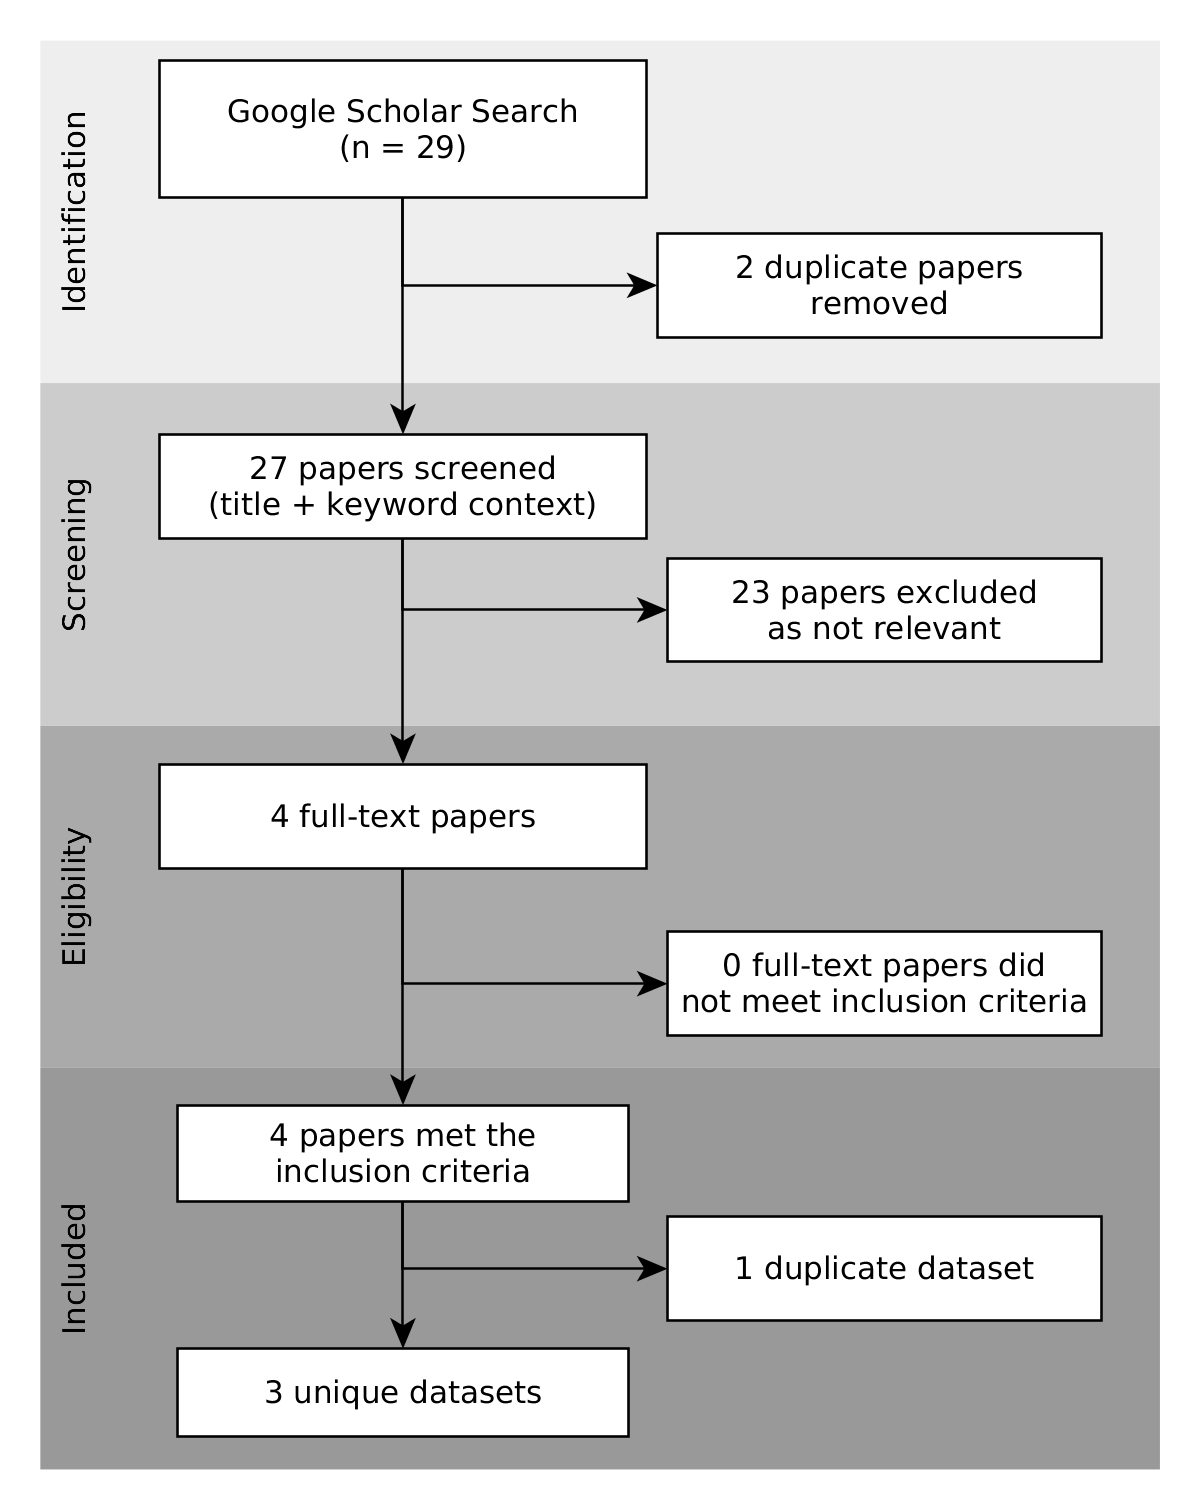
\includegraphics[width=\linewidth]{review-count-v2}
  \caption{PRISMA Flow Diagram \cite{Moher2009} showing study selection. From the literature search, the selection was refined to four relevant papers that made claims that the dataset used was non-identifiable. Two papers were grouped together that analysed the same dataset from different perspectives. All four relevant papers were subjected to scrutiny of risk of data re-identification.}
  \label{fig:prisma-review}
\end{figure}

\subsubsection{Results of individual studies}

Tables of variables (as described in Data Items \secref{sec:data-items}) for datasets 1, 2, and 3 are presented in Tables \ref{tab:de-ident-woods}, \ref{tab:de-ident-greenham}, and \ref{tab:de-ident-jacob} respectively. Improperly de-identified variables (according to the procedures in the Summary measures section, \secref{sec:summary-measures}) vulnerable to a data linkage attack are highlighted (bold red text). A full discussion of each dataset and ad-hoc analysis of other potential attacks is included in \appendixref{appendix:deidentification}.

% comparison table
\begin{landscape}

\newcommand{\highlightcell}[1]{\textbf{\textcolor{red}{#1}}}


% generated by https://www.tablesgenerator.com/
\begin{table}[]
\centering
\caption{Robertson, Woods, and Gastin \cite{Robertson2015, Woods2015}. Under 18 year old performance tests. Claims: ``non-identifiable'' data; approval by ``relevant human research ethics advisory group''; consent of ``state-based organisations''}
\label{tab:de-ident-woods}
\footnotesize % https://en.wikibooks.org/wiki/LaTeX/Fonts#Sizing_text
\hyphenpenalty=10000 % https://tex.stackexchange.com/questions/5036/how-to-prevent-latex-from-hyphenating-the-entire-document
%\begin{tabular}{lllllll}
\begin{tabular}{L{4cm}L{2.5cm}L{2.5cm}L{2.5cm}L{3cm}L{3cm}p{3cm}}
\textbf{Variable} & \textbf{Collection level} & \textbf{Collected type} & \textbf{Published level} & \textbf{Public Data?} & \textbf{Collection re\nobreakdash-identifiable?} & \textbf{Published data re\nobreakdash-identifiable?} \\
\hline
\\
Birthdate                   & Individual       & Real           & Group           & If drafted                     & Already public if drafted   & No                              \\
\\
Anthropometric measurements & Individual       & List Real      & Group           & If drafted                     & Already public if drafted   & No                              \\
\\
Physical performance        & Individual       & List Real      & Group           & \highlightcell{Only if one of top results for test} & \highlightcell{By birthdate and anthropometric measurements}                & No                              \\
\\
Drafted                     & Individual       & Categorical    & Group           & Yes                            & Identifiable                & Already Public
\end{tabular}
\end{table}

\begin{table}[]
\centering
\caption{Greenham et al. \cite{Greenham2017}. AFL team game style. Claims: ``non-identifiable player data, from identifiable team-based data-sets'' data; ethics exempt}
\label{tab:de-ident-greenham}
\raggedright
\footnotesize % https://en.wikibooks.org/wiki/LaTeX/Fonts#Sizing_text
\hyphenpenalty=10000 % https://tex.stackexchange.com/questions/5036/how-to-prevent-latex-from-hyphenating-the-entire-document
%\begin{tabular}{lllllll}
\begin{tabular}{L{4cm}L{2.5cm}L{2.5cm}L{2.5cm}L{3cm}L{3cm}p{3cm}}
\textbf{Variable} & \textbf{Collection level} & \textbf{Collected type} & \textbf{Published level} & \textbf{Public Data?} & \textbf{Collection re\nobreakdash-identifiable?} & \textbf{Published data re\nobreakdash-identifiable?} \\
\hline
\\
Team name                                                                                                                                                                                                                                                                           & Team             & String         & Team            & Yes                                                                           & Team level                  & Team Level                      \\
\\
\specialcell{Shot at goal accuracy,\\Scoring accuracy,\\Location of goal attempts (as proportion near goal),\\Passes/min,\\Passing efficiency,\\Rate of ball recovery,\\Weighted position of turnovers (per zone),\\Weighted position of turnovers weighted by score (per zone),\\Tackles/min of defence} & Team             & List Real      & Team            & Detailed statistics need licence from Champion Data (AFL statistics provider) & Team level                  & Team level                      \\
\\
Ball Speed (from video)                                                                                                                                                                                                                                                             & Individual       & Video          & Team            & Yes                                                                           & Identifiable                & Already Public                  \\
\\
Offensive-defensive numbers (from behind the goals video),\\Total numbers in forward 50 (from behind the goals video)                                                                                                                                                                & Individuals      & Video          & Team            & \highlightcell{Behind the goals video only provided to coaches}                                                      & \highlightcell{Identifiable}                & Team level
\end{tabular}
\end{table}

\begin{table}[]
\centering
\caption{Jacob et al. \cite{Jacob2016}. Genetic markers for performance. Claims: ``non-identifiable'' code; ``University granted approval'' (``Human Research and Ethics Committee approval number'' provided); direct consent of participants (and parents where under 18)}
\label{tab:de-ident-jacob}
\footnotesize % https://en.wikibooks.org/wiki/LaTeX/Fonts#Sizing_text
\hyphenpenalty=10000 % https://tex.stackexchange.com/questions/5036/how-to-prevent-latex-from-hyphenating-the-entire-document
%\begin{tabular}{lllllll}
\begin{tabular}{L{4cm}L{2.5cm}L{2.5cm}L{2.5cm}L{3cm}L{3cm}p{3cm}}
\textbf{Variable} & \textbf{Collection level} & \textbf{Collected type} & \textbf{Published level} & \textbf{Public Data?} & \textbf{Collection re\nobreakdash-identifiable?} & \textbf{Published data re\nobreakdash-identifiable?} \\
\hline
\\
Team Name           & Team             & Text            & Hidden              & Yes          & Team level                                             & Acknowledgement of team in pre-publication draft \\
\\
Genotype (from blood sample) & Individual       & {List Categorical} & Group              & No           & May correlate with family members, race, and ethnicity & No                                               \\
\\
Physical performance         & Individual       & {List Real}        & Group              & No           & By genotype                                            & No
\end{tabular}
\end{table}

\end{landscape}

\subsubsection{Synthesis of results}

Improperly de-identified variables have been highlighted in bold  red in the previous section. It was found that two of the three datasets analysed involved improper de-identification of the underlying dataset. In one case re-identifiable data were claimed non-identifiable: under 18 year old performance results are non-public (other than top performers), but the results could be linked back to the individual by birthdate and anthropometric measurements. In another case non-public identifiable video (behind the goals footage) that is only accessible to select groups (e.g. clubs) was improperly exempted from ethics review under the assumption that it was publicly available. These cases were both limited to improper de-identification of the dataset by the custodian prior to providing it to researchers. Scrutiny of the final published data (i.e. the summarised version published in the research paper) was unable to reveal any cases where it was possible to re-identify specific individuals without access to the raw dataset the researchers had access to.
%In the third dataset, while research data were collected in re-identifiable form, it obtained individual consent for this and human research ethics review.

%\subsubsection{Risk of Bias across studies}
%\subsubsection{Additional Analyses}

\subsection{Discussion}

\subsubsection{Summary of evidence}

Considering that only three datasets where examined in full, the discovery of two datasets that likely did not meet their claim as being non-identifiable suggests that many more sport studies exist where participants have not been properly de-identified in the underlying dataset. Fortunately, the published data does not appear to be re-identifiable; however, this may be due to journal page limitations which have the effect of preventing authors revealing too much, rather than a matter of careful statistical disclosure policies.

\subsubsection{Limitations}

While unable to find any cases where the published data were re-identifiable through data linkage, the public data may still be vulnerable to other forms of attacks. In \appendixref{appendix:deidentification}, a consideration is provided of other forms of attacks for some of the articles analysed; however, much like code review to catch bugs, review will catch some cases of re-identifiable data, while others may have slipped through unnoticed.

\subsubsection{Conclusions}

% Supervisor: {Question/Clarification Point: ``were not able to identify any individual players...'' by looking only at data provided? (i.e. no further linking or processing was done?? Else it weakens your primary motivation / argument.)}

In conclusion, although it was not possible to identify any individual players using the published data alone, in some cases it was possible to reduce the possible candidates by utilising information in the study in a manner contrary to the intentions of the author. However, the investigation suggests that the underlying dataset used by researchers in some of the studies was likely re-identifiable despite claims that the data were non-identifiable. This is concerning, as it can lead to re-identifiable data being used or re-shared by researchers without proper consent from the individuals to whom it pertains.

Anonymisation of team names was an unsuccessful counter-measure against attacks on participant privacy. While unintentional, ambiguity of method, or missing data served to add uncertainty which prevented identifying individuals. As research moves into an era where page count is no longer a limitation (e.g. electronic attachments), datasets are reusable (though greater access to eResearch tools to preserve datasets and facilitate reuse through capture of meta-data), methods are unambiguous (e.g. through publication of analysis source code), and data quality is high (e.g. data capture using ubiquitous sensor networks with redundancy), this uncertainty will reduce, thus formal privacy techniques will become more important to avoid revealing individual participants via ``differencing attacks'' \cite{Keefe2017}. In particular, the group of participants that were excluded from the study will reduce, possibly to single participants, and the information of these participants could be inferred through differences between overall versus clean data, or from differences between studies with slight differences of filtering techniques.

% Supervisor: {SLR is good. The way to present may need to be changed to be in line with the rest of chapter -- but content is good.}

%\subsection{Funding}

%\newpage
%\pagebreak
